\documentclass[accentcolor=tud1b,colorbacktitle,inverttitle,landscape,presentation,t]{tudbeamer}
\usepackage[utf8]{inputenc}
\usepackage[german]{babel}
\usepackage{verbatim, hyperref,multimedia}
\usepackage{graphicx, psfrag}			%to insert graphics
\usepackage{setspace}
\usepackage[active]{srcltx}
\usepackage{color}
\usepackage{subfigure}
\usepackage{listings}
\usepackage{pstricks}
\usepackage{amssymb}

\useinnertheme{default}
\usecolortheme{orchid}
\setbeamercovered{transparent}


\newcommand{\keyword}[1]{\textcolor{tudaccent}{\textbf{#1}}} 
\newcommand{\myframetitle}[2]{\frametitle{#1 \\[.2cm] \small #2}}
\newcommand{\fatitem}[1]{\item \textbf{#1}}
\newcommand{\tab}{\hspace*{0.5cm}}


\setcounter{tocdepth}{1} 

\hypersetup{
pdftitle={WebMining Exercise }, pdfauthor={F. Englert}
}


\begin{document}

\title[MGA]{\large 3. Exercise}

\author{Frank Englert, Jens Haase}
\institute{KE, TU Darmstadt}

\logo{
\includegraphics{graphics/keico}}

\date{May 2011}

\begin{titleframe}
\begin{center}
\color{tudtextaccent} \large The 3rd exercise\\[.5cm]
%\includegraphics[width=0.4\textwidth]{Graphics/spg_logo_final.eps} \\
\normalcolor \normalsize Knowlege Engineering \\
Fachbereich Informatik \\
Technische Universität Darmstadt\\[.5cm]

\textbf{Exercise Presentation:}\\
Frank Englert\\
Jens Haase
\end{center}

\end{titleframe} 

\begin{frame}[c]
	\myframetitle{3. Exercise}{Overview}
\begin{enumerate}
  \item Task 2
  \begin{itemize}
  \item ...
  \item ...
\end{itemize}
  \item Task 3
  \begin{itemize}
  \item ...
  \item ...
\end{itemize}
\end{enumerate}
\end{frame}

\begin{frame}[c]
	\myframetitle{Task 2 }{}
\begin{itemize}
  \item ...
\end{itemize}
\end{frame}


\begin{frame}[c]
	\myframetitle{Probability of Word occurences}{Zipf's law (linear scale)}
	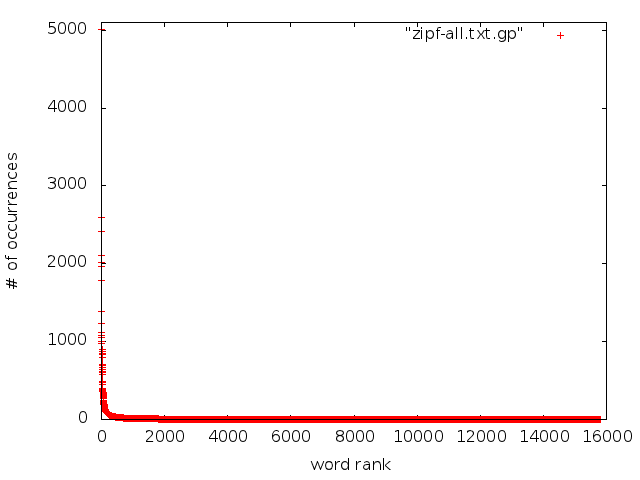
\includegraphics[scale=0.4]{../task02-04/src/main/resources/results/task3/zipf-lin.png}
\end{frame}

\begin{frame}[c]
	\myframetitle{Probability of Word occurences}{Zipf's law (log scale)}
	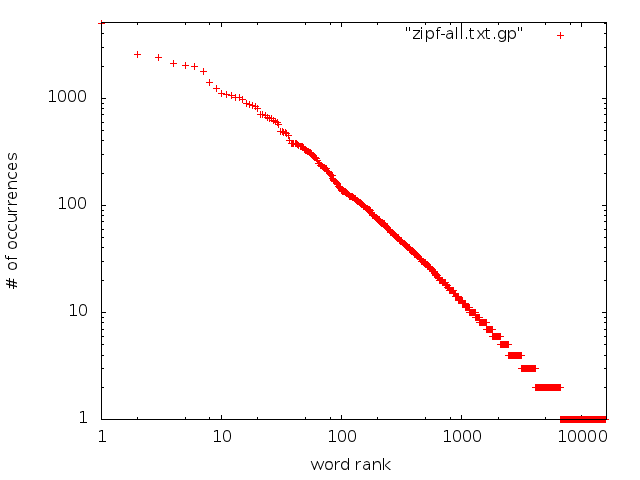
\includegraphics[scale=0.4]{../task02-04/src/main/resources/results/task3/zipf-log.png} 
\end{frame}	

\begin{frame}[c]
	\myframetitle{Probability of Word occurences}{Probability of Frequency (linear scale)}
	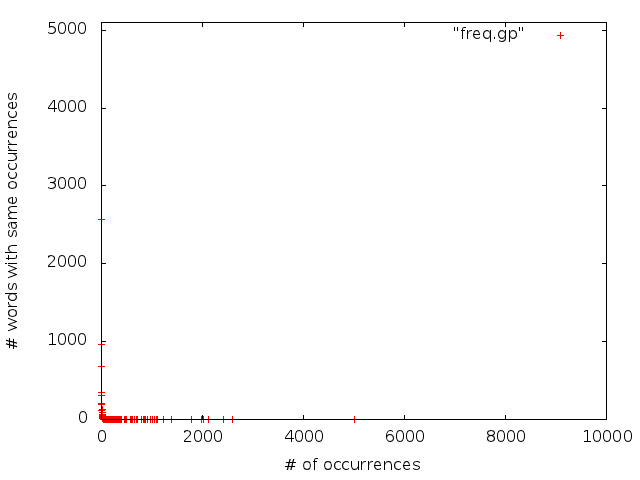
\includegraphics[scale=0.4]{../task02-04/src/main/resources/results/task3/freq-lin.png}
\end{frame}

\begin{frame}[c]
	\myframetitle{Probability of Word occurences}{Probability of Frequency (log scale)}
	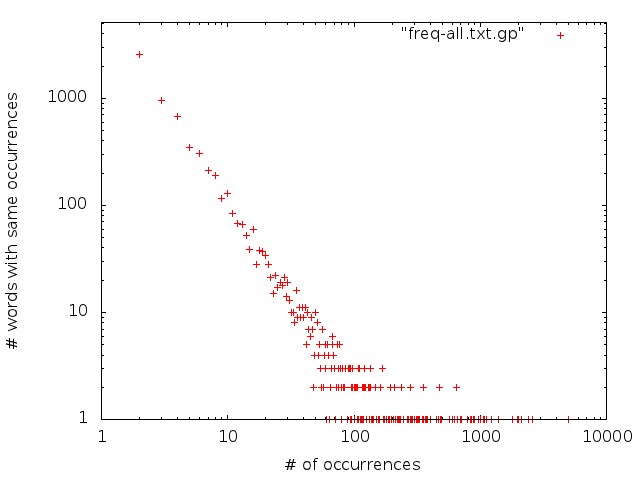
\includegraphics[scale=0.4]{../task02-04/src/main/resources/results/task3/freq-log.png} 
\end{frame}	

\end{document}
